% !TEX program = pdflatex
\documentclass[dvipsnames,aspectratio=169,handout]{beamer}
\usepackage{tikz,amsfonts}
% xcolor is typically loaded by beamer; re-loading with options may cause an option clash.
\usepackage{xcolor}
\usetikzlibrary{arrows,arrows.meta,positioning,calc,shapes}
\usepackage[absolute,overlay]{textpos}
\usepackage{multirow}
\usepackage{environ,lipsum}
\usepackage{listings}



\lstset{ 
  language=R,                     % the language of the code
  basicstyle=\scriptsize\ttfamily, % the size of the fonts that are used for the code
  columns=fullflexible,
%  numbers=left,                   % where to put the line-numbers
%  numberstyle=\tiny\color{Blue},  % the style that is used for the line-numbers
%  stepnumber=1,                   % the step between two line-numbers. If it is 1, each line
                                  % will be numbered
%  numbersep=5pt,                  % how far the line-numbers are from the code
  backgroundcolor=\color{Dandelion!15!white},  % choose the background color. You must add \usepackage{color}
  showspaces=false,               % show spaces adding particular underscores
  showstringspaces=false,         % underline spaces within strings
  showtabs=false,                 % show tabs within strings adding particular underscores
  frame=single,                   % adds a frame around the code
  rulecolor=\color{Dandelion!15!white},        % if not set, the frame-color may be changed on line-breaks within not-black text (e.g. commens (green here))
  tabsize=2,                      % sets default tabsize to 2 spaces
  captionpos=b,                   % sets the caption-position to bottom
  breaklines=true,                % sets automatic line breaking
  breakatwhitespace=false,        % sets if automatic breaks should only happen at whitespace
  keywordstyle=\color{RoyalBlue!80!black},      % keyword style
  commentstyle=\color{YellowGreen!60!black},   % comment style
  %stringstyle=\color{ForestGreen}      % string literal style
} 
\lstset{alsoletter={.,_}, morekeywords={cor.test,set.seed,dcor.test,make_tree,sample_gnm,graph,ci.test,qgraph,sample_smallworld,ciTest_table,IsingFit,averageLayout,read.table,install.packages,bdgraph,stepwise,dmod,cmod,ciTest,graph_from_adjacency_matrix,mvrnorm,CondIndTest,as.data.frame,chisq.test,gnm,smallworld,ug,dag,edge,as.igraph,degree,diameter,centrality,cluster,betweenness,at}
}


\newcommand{\customframefont}[1]{
\setbeamertemplate{itemize/enumerate body begin}{#1}
\setbeamertemplate{itemize/enumerate subbody begin}{#1}
}

\NewEnviron{framefont}[1]{
\customframefont{#1} % for itemize/enumerate
{#1 % For the text outside itemize/enumerate
\BODY
}
\customframefont{\normalsize}
}



%%%%%%%%% BASICS
\usenavigationsymbolstemplate{}

\setbeamertemplate{frametitle}
  {\begin{centering}\smallskip
   \insertframetitle\par
   \smallskip\end{centering}}
\setbeamersize{text margin left=.2cm,text margin right=.2cm} 
\setbeamertemplate{itemize item}{$\bullet$}
\setbeamertemplate{navigation symbols}{}
\setbeamertemplate{footline}[text line]{%
    \hfill\strut{%
        \scriptsize\sf\color{black!60}%
        \quad\insertframenumber/\inserttotalframenumber
    }%
    \hfill
    
}

%%%%%%%%% COLOR THEME

% Define some colors:
\definecolor{asparagus}{rgb}{0.53, 0.66, 0.42}
\definecolor{DarkFern}{HTML}{407428}
\definecolor{DarkCharcoal}{HTML}{4D4944}
\colorlet{Fern}{DarkFern!85!white}
\colorlet{Charcoal}{DarkCharcoal!85!white}
\colorlet{LightCharcoal}{Charcoal!50!white}
\definecolor{Important}{RGB}{234,122,133}
\colorlet{AlertColor}{Melon!30!red}
\colorlet{DarkRed}{red!70!black}
\colorlet{DarkBlue}{blue!70!black}
\colorlet{DarkGreen}{green!70!black}
\definecolor{ExampleBlue}{RGB}{230,242,255}
\setbeamercolor{examplepanel}{fg=black,bg=ExampleBlue}
% Use the colors:
\setbeamercolor{title}{fg=Fern}
\setbeamercolor{frametitle}{fg=Fern}
\setbeamercolor{normal text}{fg=Charcoal}
\setbeamercolor{block title}{fg=black,bg=Fern!15!white}
\setbeamercolor{block body}{fg=black,bg=Fern!15!white}
%\setbeamercolor{block body alerted}{fg=black,bg=Goldenrod!5!white}
%\setbeamercolor{block body example}{fg=black,bg=Fern!15!white}
\setbeamercolor{alerted text}{fg=AlertColor}
\setbeamercolor{itemize item}{fg=Charcoal}
\setbeamercolor{framesource}{fg=gray}
\setbeamerfont{framesource}{size=\tiny}

%%%%% DEFINITIONS

\DeclareMathOperator{\sgn}{sgn}
\DeclareMathOperator{\rank}{rank}
\DeclareMathOperator{\D}{D}
\DeclareMathOperator{\cov}{cov}
\DeclareMathOperator{\cor}{cor}
\DeclareMathOperator{\var}{var}
\DeclareMathOperator{\tr}{tr}
\DeclareMathOperator{\pa}{pa}
\DeclareMathOperator{\de}{de}
\DeclareMathOperator{\nd}{nd}

\newcommand{\bx}{\mathbf{x}}
\newcommand{\by}{\mathbf{y}}
\newcommand{\C}{\mathbb{C}}
\newcommand{\cC}{\mathcal{C}}
\newcommand{\E}{\mathbb{E}}
\newcommand{\cE}{\mathcal{E}}
\newcommand{\cI}{\mathcal{I}}
\newcommand{\J}{\rm {J}}
\newcommand{\cL}{\mathcal{L}}
\newcommand{\cM}{\mathcal{M}}
\newcommand{\N}{\mathbb{N}}
\renewcommand{\P}{\mathbb{P}}
\newcommand{\Q}{\mathbb{Q}}
\newcommand{\R}{\mathbb{R}}
\renewcommand{\S}{\mathbb{S}}
\newcommand{\cS}{\mathcal{S}}
\newcommand{\cX}{\mathcal{X}}
\newcommand{\Z}{\mathbb{Z}}
\newcommand{\bs}{\boldsymbol}
\newcommand{\imp}[1]{\textcolor{DarkRed}{\textbf{#1}}}
\newcommand{\why}{\textcolor{WildStrawberry}{{\textsc{why?}}}}
\newcommand{\indep}{\mbox{\,$\perp\!\!\!\perp$\,}}
\newcommand{\mtp}{{\rm MTP}_{2}}
\newcommand{\eps}{\varepsilon}

\def\imagetop#1{\vtop{\null\hbox{#1}}}
\def\house{\hbox{\kern3pt \vbox to12pt{}% 
   \pdfliteral{q 0 0 m 0 5 l 5 10 l 10 5 l 10 0 l 7 0 l 7 5 l 3 5 l 3 0 l f
               1 j 1 J -2 5 m 5 12 l 12 5 l S Q }%
   \kern 13pt}}

%source for images
\newcommand{\source}[1]{\begin{textblock*}{4cm}(8.7cm,8.6cm)
    \begin{beamercolorbox}[ht=0.5cm,right]{framesource}
        \usebeamerfont{framesource}\usebeamercolor[fg]{framesource} Source: {#1}
    \end{beamercolorbox}
\end{textblock*}}

%%% TITLE INFO



\institute{\begin{center}
  \IfFileExists{LOGOstats.png}{\raisebox{-0.5\height}{
\includegraphics[scale=.27]{LOGOstats.png}}}{} 
  \hspace{1mm}
  \IfFileExists{LOGOBSE.jpg}{\raisebox{-0.5\height}{
\includegraphics[scale=.08]{LOGOBSE.jpg}}}{} 
\end{center}}


\setbeamercolor{notabene}{fg=black!50!white,bg=Gray!10!white}
\setbeamercolor{important}{fg=red!50!white,bg=red!7!white}
\setbeamercolor{goldbox}{fg=black!50!white,bg=Goldenrod!7!white}
\setbeamercolor{result}{fg=black!60!white,bg=OliveGreen!4!white}
% \begin{beamercolorbox}[wd=\paperwidth,sep=7pt]{important}	
%	%\end{beamercolorbox}


\title{Advanced techniques in applied economics}
\subtitle{Lecture 1: Conditional independence as structure}
\author{Piotr Zwiernik}
\date{Spring 2026}

\begin{document}

% ------------------------------------------------------------
% Title
% ------------------------------------------------------------

\begin{frame}[plain,noframenumbering]
\titlepage
\end{frame}

% ------------------------------------------------------------
% About the course
% ------------------------------------------------------------

\section{About the course}

\begin{frame}[plain,noframenumbering]{}
\begin{center}
{\huge \textcolor{DarkRed}{About the course}}
\end{center}
\end{frame}

\begin{frame}{Why this course?}
\begin{itemize}
    \item We live in a world of \alert{high-dimensional dependence}.
    \item Standard tools often break down when too many variables interact.
    \item Economists increasingly work with data where \alert{structure} matters:
    networks, latent factors, strategic interactions, and policy spillovers.
\end{itemize}
\vspace{-6mm}
\begin{columns}[T]
\begin{column}{0.32\textwidth}
    \begin{center}
        \textcolor{DarkBlue}{\textbf{1. Efficiency}}
    \end{center}
    \small
    \textbf{Conditional independence (CI) } tells us what can be ignored.
    This can turn an impossible problem into a tractable one.
\end{column}
\quad
\begin{column}{0.32\textwidth}
    \begin{center}
        \textcolor{DarkBlue}{\textbf{2. Interpretation}}
    \end{center}
    \small
    \textbf{Graphical structure} helps separate direct from indirect relations.
    This is crucial for causal and policy reasoning.
\end{column}
\begin{column}{0.32\textwidth}
    \begin{center}
        \textcolor{DarkBlue}{\textbf{3. Expressivity}}
    \end{center}
    \small
    \textbf{Latent variables} capture hidden drivers such as confounders,
    common shocks, market factors, and unobserved heterogeneity.
\end{column}
\end{columns}
\medskip
\begin{beamercolorbox}[wd=\textwidth,sep=3pt,center,rounded=true,shadow=true]{important}
{\Large \textbf{Core message}}\\[1mm]
\alert{Conditional independence + graphs + latent variables = scalable structure for modern empirical work}
\end{beamercolorbox}
\end{frame}

\begin{frame}{Course structure and objectives}
\small
\begin{columns}[T]
\begin{column}{0.50\textwidth}
\textbf{Format}
\begin{itemize}
    \item \textbf{8 content lectures + 2 project sessions}
    \item Mixture of theory, examples, and hands-on implementation
\end{itemize}

\textbf{Tools}
\begin{itemize}
    \item Mathematical derivations and visual intuition
    \item \texttt{R} examples using packages such as
    \texttt{huge}, \texttt{glasso}, \texttt{pcalg}, \texttt{dagitty}
\end{itemize}
\end{column}

\begin{column}{0.47\textwidth}
\begin{block}{\small \imp{Applied economics angle}}
I will try to connect the theory to problems economists care about:
\begin{itemize}
    \item \small causal identification and policy design,
    \item \small financial and macroeconomic dependence,
    \item \small latent heterogeneity and confounding,
    \item \small interference and network spillovers.
\end{itemize}
\end{block}
\end{column}
\end{columns}

\vspace{1mm}

\begin{alertblock}{Assessment}
The main assessment is a research project. You may choose:
\begin{itemize}
    \item \textbf{Applied project:} empirical analysis of a structured model.
    \item \textbf{Methods project:} deeper study of one model class or algorithm.
\end{itemize}
\end{alertblock}
\end{frame}

\begin{frame}{Roadmap for today}
\begin{enumerate}
    \item Basic notions: joint, marginal, conditional distributions\\[3mm]
    \item Independence and conditional independence\\[3mm]
    \item Regression and the Gaussian bridge\\[3mm]
    \item Why conditioning can change conclusions\\[3mm]
    \item Testing dependence in real data\\[3mm]
\end{enumerate}

\vspace{2mm}

\begin{beamercolorbox}[wd=\textwidth,sep=7pt,center,rounded=true,shadow=true]{important}
Conditioning is not a technicality --- it is often the whole story.
\end{beamercolorbox}
Reading:\\[.1cm]
{S. H\o jsgaard, D. Edwards, S. Lauritzen, \emph{Graphical Models with R}}.\\
{R. Alexander, \emph{Telling stories with data}, Chapter 15.}

\end{frame}

% ------------------------------------------------------------
% Foundations
% ------------------------------------------------------------

\section{Conditional independence}

\begin{frame}[plain,noframenumbering]{}
\begin{center}
{\Huge \textcolor{DarkRed}{Part 1: Conditional independence}}
\end{center}
%\vspace{1cm}
%\begin{center}
%Reading:\\[.1cm]
%[\alert{S. H\o jsgaard, D. Edwards, S. Lauritzen, \emph{Graphical Models with R}}]
%\end{center}
\end{frame}

\subsection{Basic concepts}

\begin{frame}{Random vectors and joint distributions}
Let $(X,Y)$ be a random vector.

\begin{alertblock}{Joint distribution}
It describes the full probabilistic behaviour of $(X,Y)$.
\begin{itemize}
    \item \textbf{Continuous case:} density $f_{XY}(x,y)$
    \item \textbf{Discrete case:} probability mass function
    \[
    f_{XY}(x,y)=\P(X=x,Y=y)
    \]
\end{itemize}
\end{alertblock}\vspace{-4mm}
\begin{block}{}
\small A joint distribution describes how variables move \emph{together}, e.g.:\\[3mm]
\begin{minipage}{7cm}
\begin{itemize}
    \item inflation and unemployment,\\[-2mm]
    \item returns on two assets,\\[-2mm]
\end{itemize}	
\end{minipage}
\begin{minipage}{7cm}
\begin{itemize}
    \item income and consumption,\\[-2mm]
    \item treatment assignment and outcomes.
\end{itemize}	
\end{minipage}
\end{block}
\end{frame}

\begin{frame}{Marginal distributions}
Marginals are obtained by summing or integrating out the other variable from $f_{XY}(x,y)$.

\begin{columns}[T]
\begin{column}{0.53\textwidth}
\begin{alertblock}{Marginal distribution of $X$}
\textbf{Continuous case:}
\[
f_X(x)=\int_{\mathbb R} f_{XY}(x,y)\,dy
\]

\textbf{Discrete case:}
\[
f_X(x)=\sum_y f_{XY}(x,y)=\P(X=x)
\]
\end{alertblock}
\end{column}

\begin{column}{0.43\textwidth}
\begin{center}
\begin{tikzpicture}[scale=0.7]
\draw[->,thick] (0,0) -- (4,0) node[right] {$x$};
\draw[->,thick] (0,0) -- (0,3.8) node[above] {$y$};

\fill[blue!12] (2,2) ellipse (1.6 and 1.1);
\fill[blue!22] (2,2) ellipse (1.25 and 0.85);
\fill[blue!35] (2,2) ellipse (0.9 and 0.6);
\fill[blue!50] (2,2) ellipse (0.5 and 0.3);

\draw[dashed,very thick,BrickRed] (2.9,0) -- (2.9,3.5);
\node[BrickRed] at (2.9,-0.35) {$x$};

\node at (1.5,3.4) {\small joint density};
\node at (2,-0.85) {\small collect mass in the vertical slice};
\end{tikzpicture}
\end{center}
\end{column}
\end{columns}
%\begin{block}{Interpretation}
%To get the marginal law of $X$, we ignore the exact value of $Y$ and collect all probability mass compatible with $X=x$.
%\end{block}

\end{frame}

\begin{frame}{Conditional distributions}
A conditional distribution tells us how one variable behaves once another variable is known.
\begin{alertblock}{Conditional distribution}
For all $x$ such that $f_X(x)>0$,
\[
f_{Y|X}(y|x)=\frac{f_{XY}(x,y)}{f_X(x)}.
\]
In the discrete case this becomes
\[
\P(Y=y\mid X=x)=\frac{\P(X=x,Y=y)}{\P(X=x)}.
\]
\end{alertblock}
\vspace{-4mm}
\begin{block}{}
\small Conditioning means that we restrict attention to a subpopulation.\\[3mm]
\begin{minipage}{7cm}
	\begin{itemize}
    \item among employed workers,\\[-2mm]
    \item among treated units,\\[-2mm]
\end{itemize}
\end{minipage}\begin{minipage}{8cm}
	\begin{itemize}
    \item among firms in distress,\\[-2mm]
    \item among borrowers with a given credit score.
\end{itemize}
\end{minipage}
\end{block}
\end{frame}

\begin{frame}{Note: Be careful interpreting conditional probabilities}
\begin{block}{Scenario: AI fraud detection}
An algorithm flags fraudulent transactions ($F$).
It catches 90\% of fraud, and correctly labels 90\% of clean transactions.
\end{block}

\begin{columns}[T]
\begin{column}{0.45\textwidth}
\centering
\textbf{Joint probabilities}\\[1mm]
\begin{tabular}{l|cc}
& Fraud ($F$) & Clean ($F^c$) \\ \hline
Flag (+)    & 0.009 & 0.099 \\
No flag (-) & 0.001 & 0.891
\end{tabular}
\end{column}

\begin{column}{0.48\textwidth}
\begin{itemize}
    \item \textbf{Sensitivity:} $\P(+\mid F)=0.9$
    \item \textbf{Specificity:} $\P(-\mid F^c)=0.9$
    \item \textbf{Prevalence:} $\P(F)=0.01$
\end{itemize}
\end{column}
\end{columns}

\medskip

\begin{alertblock}{Direction of conditioning matters}
If a transaction is flagged, the probability that it is actually fraud equals
\[
\P(F\mid +)=\frac{0.009}{0.009+0.099}\approx 0.083.
\]
So even a strong test may generate many false alarms when the event is rare.
\end{alertblock}
\end{frame}


\begin{frame}{Independence}
\begin{block}{}
$X$ and $Y$ are \imp{independent}, written $X\indep Y$, if and only if\\[3mm]
\qquad\qquad\qquad\qquad\qquad$
f_{XY}(x,y)=f_X(x)f_Y(y)
\qquad\mbox{for all }x,y.
$
\end{block}

\begin{alertblock}{Equivalent reformulation}
$X\indep Y$ if and only if
\[
f_{Y|X}(y|x)=f_Y(y)
\qquad\mbox{for all }x\mbox{ such that }f_X(x)>0.
\]
So learning $X$ does not change the distribution of $Y$.
\end{alertblock}

\begin{beamercolorbox}[wd=\textwidth,sep=8pt,center,rounded=true,shadow=true]{important}
Independence means that knowing $X$ does not help to predict $Y$.
\end{beamercolorbox}
\end{frame}


\begin{frame}{Conditional expectation and mean independence}
The conditional expectation of $Y$ given $X=x$ is
\[
\E[Y\mid X=x]=\int y\,f_{Y|X}(y\mid x)\,dy.
\]

\begin{block}{}
\qquad $\E[Y\mid X]$ is the best predictor of $Y$ from $X$ under squared loss (\imp{regression function}).\\[2mm]
\end{block}

\begin{alertblock}{Mean independence}
We say that $X$ and $Y$ are mean independent if $\E[X|Y]=\E[X]$ and $\E[Y|X]=\E[Y]$.
\end{alertblock}
\medskip
\begin{beamercolorbox}[wd=\textwidth,sep=7pt,center,rounded=true,shadow=true]{important}
Mean independence is strictly weaker than independence.
\end{beamercolorbox}
\end{frame}

\begin{frame}{Conditional independence}
$X$ and $Y$ are \imp{independent given $Z$}, written $X\indep Y\mid Z$, if
\[
f_{XY|Z}(x,y|z)=f_{X|Z}(x|z)f_{Y|Z}(y|z)
\qquad\mbox{for all }x,y, \mbox{and }z.
\]

\begin{block}{Equivalently $f_{Y|XZ}(y|x,z)=f_{Y|Z}(y|z)$}
Once $Z$ is known, learning $X$ gives no additional information about $Y$.
\end{block}

\begin{alertblock}{Screening off}
In a chain\;\;\;$
X \longrightarrow Z \longrightarrow Y,\;\;
$
the middle variable $Z$ can screen off $X$ from $Y$:
\[
X\indep Y\mid Z.
\]
\end{alertblock}\vspace{-3mm}
\begin{beamercolorbox}[wd=\textwidth,sep=8pt,center,rounded=true,shadow=true]{important}
Conditional independence captures absence of a direct link.
\end{beamercolorbox}
\end{frame}




\begin{frame}{Why economists should care}
Conditional independence is everywhere in applied work.
\begin{columns}[T]
\begin{column}{0.46\textwidth}
\begin{block}{Causal identification}
Unconfoundedness is a conditional independence statement:\\[1mm]
\qquad\qquad\qquad $
(Y(1),Y(0))\indep D\mid X.
$
\end{block}

\begin{block}{Finance and macro}
Sparse dependence means that many variables are unrelated once the right controls are included.
\end{block}
\end{column}

\begin{column}{0.46\textwidth}
\begin{block}{Selection problems}
Apparent differences may disappear or reverse after conditioning on the right variables.
\end{block}

\begin{block}{Latent structures}
Many models are built by asserting that certain variables become independent once hidden factors are known.
\end{block}
\end{column}
\end{columns}

\vspace{2mm}

\begin{beamercolorbox}[wd=\textwidth,sep=7pt,center,rounded=true,shadow=true]{important}
In empirical work, assumptions are often best understood as CI restrictions.
\end{beamercolorbox}
\end{frame}

% ------------------------------------------------------------
% Regression and Gaussian bridge
% ------------------------------------------------------------

\section{Regression and Gaussian bridge}

\begin{frame}[plain,noframenumbering]{}
\begin{center}
{\Huge \textcolor{DarkRed}{Part 2: Regression and the Gaussian bridge}}
\end{center}
\end{frame}

\begin{frame}{CI and the regression function}
Suppose
\[
Y=\beta X+\gamma Z+\varepsilon,
\qquad \varepsilon\indep (X,Z).
\]
\vspace{-5mm}
\begin{block}{}
If $\beta=0$, then
\[
Y\indep X\mid Z.
\]
So after controlling for $Z$, the variable $X$ no longer matters.
\end{block}

\begin{alertblock}{Caution}
If we only assume $\E[\varepsilon\mid X,Z]=0$, then $\beta=0$ implies only that the \emph{conditional mean} does not depend on $X$.
This does \textbf{not} imply full conditional independence in general.
\end{alertblock}
\end{frame}

\begin{frame}{The multivariate normal distribution}

\begin{block}{}
A random vector $X=(X_1,\ldots,X_m)$ is Gaussian, written
$
X\sim \mathcal N_m(\mu,\Sigma)$, if the density is\[
f(x)=\frac{1}{(2\pi)^{m/2}|\Sigma|^{1/2}}
\exp\left\{-\frac12 (x-\mu)^\top\Sigma^{-1}(x-\mu)\right\},
\]
where $\mu\in\mathbb R^m$ is the mean vector and  $\Sigma\in\mathbb S_+^m$ is the covariance matrix.
\end{block}

\begin{alertblock}{Why this matters}
In Gaussian models, many conditional independence questions become algebraic.
This is why Gaussian graphical models are so useful.
\end{alertblock}
\end{frame}

\begin{frame}{Gaussian marginals $X\sim \mathcal N(\mu,\Sigma)$}
Partition $X$ into two subvectors:
\[
X=
\begin{pmatrix}
X_A\\ X_B
\end{pmatrix},
\qquad
\mu=
\begin{pmatrix}
\mu_A\\ \mu_B
\end{pmatrix},
\qquad
\Sigma=
\begin{pmatrix}
\Sigma_{AA} & \Sigma_{AB}\\
\Sigma_{BA} & \Sigma_{BB}
\end{pmatrix}.
\]

\begin{block}{Marginal law for Gaussians}
\qquad\qquad\qquad\qquad\qquad\qquad\qquad$X_A\sim \mathcal N(\mu_A,\Sigma_{AA})$.
\end{block}
\vspace{-5mm}
\begin{alertblock}{}
To study $X_A$ alone, we simply \emph{drop} the other coordinates.
No integration is needed.
\end{alertblock}
\ \\
\begin{beamercolorbox}[wd=\textwidth,sep=7pt,center,rounded=true,shadow=true]{important}
Gaussian families are closed under marginalization.
\end{beamercolorbox}
\end{frame}

\begin{frame}{Gaussian conditionals}
Under the same partition,
the conditional distribution of $X_A$ given $X_B=x_B$ is Gaussian:
\begin{align*}
\E[X_A\mid X_B=x_B]
&=
\mu_A+\Sigma_{AB}\Sigma_{BB}^{-1}(x_B-\mu_B),\\[1mm]
\var(X_A\mid X_B=x_B)
&=
\Sigma_{AA}-\Sigma_{AB}\Sigma_{BB}^{-1}\Sigma_{BA}.
\end{align*}

\begin{block}{Note that:}
\qquad$\bullet$ The conditional mean is linear in $x_B$.

\qquad$\bullet$ The conditional covariance matrix does not depend on $x_B$!
\end{block}

\ 
\begin{beamercolorbox}[wd=\textwidth,sep=7pt,center,rounded=true,shadow=true]{important}
Under Gaussianity, conditioning preserves Gaussianity and linearity.
\end{beamercolorbox}
\end{frame}

\begin{frame}{A special Gaussian feature}
For general distributions,
\[
\cov(X_A,X_B)=0
\]
does \textbf{not} imply independence.

\medskip

For jointly Gaussian vectors, however, we have the equivalence
\[
X_A\indep X_B
\qquad\Longleftrightarrow\qquad
\Sigma_{AB}=0.
\]

\begin{block}{Practical implication}
Many tools exploit Gaussian logic,
even when this is not made explicit.\\
\qquad e.g. some ``independence'' tests test zero covariance.
\end{block}
\end{frame}

\begin{frame}{The precision matrix}
The \alert{precision matrix} is
\[
K=\Sigma^{-1}.
\]
Partition it in the same way:
\[
K=
\begin{pmatrix}
K_{AA} & K_{AB}\\
K_{BA} & K_{BB}
\end{pmatrix}.
\]

Using block matrix inversion and the Schur complement, one obtains
\[
\var(X_A\mid X_B=x_B)=K_{AA}^{-1}.
\]

\begin{alertblock}{Why this is important}
\quad $\bullet$ The covariance matrix describes marginal dependence.

\quad $\bullet$ The precision matrix describes conditional dependence.
\end{alertblock}
\end{frame}

\begin{frame}{Precision matrix and conditional independence}
Let $X=(X_1,\ldots,X_m)^\top\sim\mathcal N_m(\mu,\Sigma)$ and let $K=\Sigma^{-1}$.

\begin{beamercolorbox}[wd=\textwidth,sep=8pt,center,rounded=true,shadow=true]{important}
For Gaussian data,
\[
X_i\indep X_j\mid X_{\{1,\ldots,m\}\setminus\{i,j\}}
\qquad\Longleftrightarrow\qquad
K_{ij}=0.
\]
\end{beamercolorbox}

\begin{block}{Interpretation}
A zero off-diagonal entry in the precision matrix means:
once all other variables are controlled for,
there is no remaining direct relation between $X_i$ and $X_j$.
\end{block}

\begin{alertblock}{This is the bridge to graphs}
Later we will encode these zeros by missing edges in an undirected graph.
\end{alertblock}
\end{frame}

\begin{frame}{Partial correlation}
For three variables $X,Y,Z$, the partial correlation is
\[
\rho_{X,Y\cdot Z}
=
\frac{\rho_{X,Y}-\rho_{X,Z}\rho_{Y,Z}}
{\sqrt{(1-\rho_{X,Z}^2)(1-\rho_{Y,Z}^2)}}.
\]

\begin{block}{Meaning}
It measures the residual linear association between $X$ and $Y$
after removing the linear effect of $Z$.
\end{block}

\begin{alertblock}{Regression interpretation}
$\rho_{X,Y\cdot Z}=0$ if and only if in the linear regression of $X$ on $Y$ and $Z$,
the coefficient of $Y$ is zero.
\end{alertblock}

\begin{block}{In the Gaussian case}
Zero partial correlation is equivalent to conditional independence.
\end{block}
\end{frame}

%\begin{frame}{Partial correlation and the precision matrix}
%If $X=(X_1,\ldots,X_m)$ has covariance matrix $\Sigma$ and precision matrix $K=\Sigma^{-1}$, then
%\[
%\rho_{X_i,X_j\cdot X_{\{1,\ldots,m\}\setminus\{i,j\}}}
%=
%-\frac{K_{ij}}{\sqrt{K_{ii}K_{jj}}}.
%\]
%
%\begin{block}{Regression link}
%In the linear regression of $X_i$ on the remaining variables,
%the coefficient of $X_j$ is
%\[
%\beta_{ij}=-\frac{K_{ij}}{K_{ii}}.
%\]
%\end{block}
%
%\begin{beamercolorbox}[wd=\textwidth,sep=7pt,center,rounded=true,shadow=true]{important}
%In Gaussian models, zeros in the precision matrix are zeros in direct predictive content.
%\end{beamercolorbox}
%\end{frame}

\begin{frame}{Economic interpretation of sparse precision matrices}
Suppose $X$ is a vector of many macro or financial variables.

\begin{block}{Dense covariance}
A dense covariance matrix means many variables move together marginally.
This may simply reflect common shocks.
\end{block}

\begin{block}{Sparse precision}
A sparse precision matrix means that once the rest is controlled for,
only a few pairs remain directly related.
\end{block}

\begin{alertblock}{Examples}
\begin{itemize}
    \item financial contagion networks,
    \item interbank or input-output dependence,
    \item psychometric and preference networks,
    \item sparse dependence in large macro panels.
\end{itemize}
\end{alertblock}
\end{frame}

% ------------------------------------------------------------
% Why conditioning matters
% ------------------------------------------------------------

\section{Why conditioning matters}

\begin{frame}[plain,noframenumbering]{}
\begin{center}
{\Huge \textcolor{DarkRed}{Part 3: Why conditioning matters}}
\end{center}
\end{frame}

\begin{frame}{A big lesson}
Simpson's paradox and Berkson's paradox are not curiosities.

\medskip

\begin{center}
\Large \textbf{Statistical conclusions depend on what we condition on.}
\end{center}

\medskip

\begin{itemize}
    \item The same data may suggest opposite conclusions under different conditioning sets.
    \item Conditioning can remove or add dependence.
    \item Positive association can become negative after conditioning and vice versa.
\end{itemize}

\vspace{2mm}

\begin{beamercolorbox}[wd=\textwidth,sep=7pt,center,rounded=true,shadow=true]{important}
Conditioning can clarify a relationship, but it can also manufacture one.
\end{beamercolorbox}
\end{frame}

\begin{frame}{An applied economics version of Simpson's paradox}
Suppose we compare outcomes across two groups, say $A$ and $B$.

\begin{block}{}
\textbf{Naive comparison:} We observe
\[
\E[Y\mid G=B]>\E[Y\mid G=A].
\]
This might tempt us to conclude that group $B$ does better.
\end{block}

\begin{alertblock}{But what if the groups differ in skill, education, sector, age, or risk exposure?}
Then the marginal comparison may mix:\\[2mm]
\qquad $\bullet$ composition effects, \qquad $\bullet$ treatment effects, \qquad $\bullet$ selection effects.
\end{alertblock}

\begin{block}{Lesson: Before interpreting an association, ask}
\qquad \qquad \qquad \qquad \qquad \qquad \textbf{What should I condition on?}\\[1mm]
\end{block}
\end{frame}

\begin{frame}{Example 1: Kidney stones}
Ignoring confounding can lead to wrong causal conclusions.

\begin{itemize}
\item Study of $700$ patients with kidney stones [Charig,1986].
\item Two treatments:
\begin{itemize}
  \item $T=a$: open surgery
  \item $T=b$: percutaneous nephrolithotomy
\end{itemize}
\item Overall recovery rates:
\begin{itemize}
  \item $\mathbb P(R=1 \mid T=a) = 0.78$
  \item $\mathbb P(R=1 \mid T=b) = 0.83$
\end{itemize}
\end{itemize}

\medskip
\alert{Based on overall rates, treatment $b$ looks better.}

\end{frame}


\begin{frame}{Conditioning on stone size}

Patients can be divided into two groups: small/large kidney stones

\medskip
\begin{center}
\begin{tabular}{lccc}
\hline
 & Overall & Small stones & Large stones \\
\hline
Treatment $a$ & $78\%$ & \alert{$93\%$} & \alert{$73\%$} \\
Treatment $b$ & \alert{$83\%$} & $87\%$ & $69\%$ \\
\hline
\end{tabular}
\end{center}

\medskip
\alert{Treatment $a$ is better in both subgroups.}

\medskip
Stone size acts as a \textbf{confounder}:
\begin{itemize}
\item Large stones are harder to treat
\item More severe cases were more likely assigned to treatment $a$
\end{itemize}

\end{frame}


\begin{frame}[label=SP]{Example 2: UC Berkeley admissions example}
		The admission figures of the grad school at UC Berkeley in 1973: 8442 (44\%) men, 4321 (35\%) women admitted.\\[.3cm] 
\pause		The same data conditioned on the department are:\\[.3cm]
\hspace{.7cm}\begin{tabular}{|c|c|c|c|c|}
\hline
\multirow{2}{*}{Department} & \multicolumn{2}{c|}{Men}   & \multicolumn{2}{c|}{Women} \\ \cline{2-5} 
                            & Applicants & Admitted       & Applicants & Admitted       \\ \hline
A                           & 825        & 62\%          & 108        & \textbf{82\%} \\ \hline
B                           & 560        & 63\%          & 25         & \textbf{68\%} \\ \hline
C                           & 325        & \textbf{37\%} & 593        & 34\%          \\ \hline
D                           & 417        & 33\%          & 375        & \textbf{35\%} \\ \hline
E                           & 191        & \textbf{28\%} & 393        & 24\%          \\ \hline
F                           & 373        & 6\%           & 341        & \textbf{7\%}  \\ \hline
\end{tabular}
\medskip

``Measuring bias is harder than is usually assumed, and the evidence is sometimes contrary to expectation.''\\[.3cm] \tiny(Bickel et al,  \textit{Sex Bias in Graduate Admissions: Data From Berkeley}, Science, 1975) 
\end{frame}




\begin{frame}{Simpson's paradox: Ilustration}
	\begin{center}
		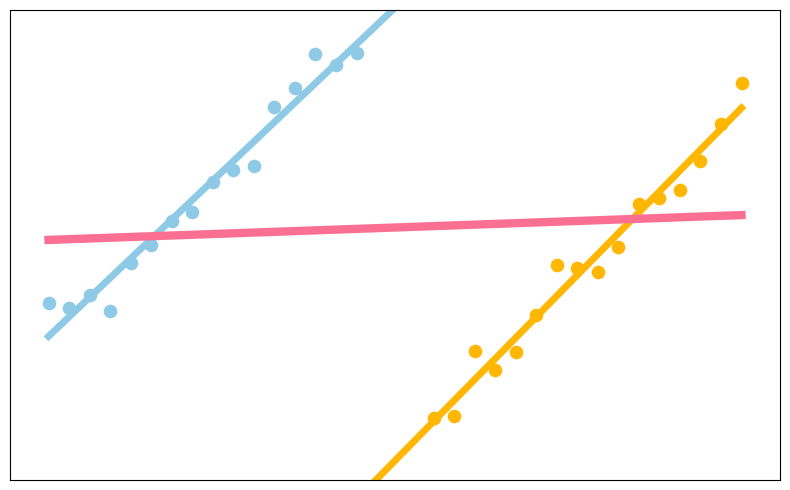
\includegraphics[scale=.5]{pics/simpson.png}
	\end{center}
\end{frame}







\begin{frame}{Berkson's paradox: conditioning on a collider}
Suppose Looks ($X$) and Personality ($Y$) are independent in the population.

\medskip

You only date people who are either attractive or nice.
Then being selected into your dating pool depends on both variables.

\begin{center}
\begin{tikzpicture}[
node distance=1cm,
every node/.style={
circle,
draw,
very thick,
minimum size=6mm,
font=\bfseries
},
edge/.style={->,very thick},
Xstyle/.style={fill=blue!20},
Ystyle/.style={fill=green!20},
Sstyle/.style={fill=orange!25}
]
\node[Xstyle] (X) {$X$};
\node[Ystyle] (Y) [right=1.2cm of X] {$Y$};
\node[Sstyle] (S) [below=1cm of $(X)!0.5!(Y)$] {$S$};
\draw[edge] (X) -- (S);
\draw[edge] (Y) -- (S);
\end{tikzpicture}
\end{center}

\begin{alertblock}{Lesson}
Even if $X\indep Y$ in the population,
conditioning on the common effect $S$ may induce dependence:
\[
X \not\!\!\!\indep Y\mid S.
\]
\end{alertblock}
\end{frame}

\begin{frame}{Economic versions of Berkson's paradox}
Selection can create misleading dependence in many economic settings.

\begin{block}{Examples}
\begin{itemize}
    \item \textbf{Wage and job satisfaction} among workers who \alert{stay} in a demanding sector.  \\
    {\small Workers with lower wages may stay only if job satisfaction is high, and vice versa.}

%    \item \textbf{Risk tolerance and realized returns} among investors who \alert{choose} a risky asset class.  \\
%    {\small     Entry into the asset class  may depend on both risk tolerance and expected performance.}

    \item \textbf{Ability and family background} among students \alert{admitted} to a selective program. \\ 
    {\small Students with weaker background may enter only if ability is very high, and vice versa.}
\end{itemize}
\end{block}

\begin{alertblock}{General lesson}
These variables may be weakly related, or even unrelated, in the full population.
But after conditioning on the selection event, they can become associated.
\end{alertblock}

\begin{beamercolorbox}[wd=\textwidth,sep=7pt,center,rounded=true,shadow=true]{important}
Conditioning on a consequence can create dependence that was not there before.
\end{beamercolorbox}
\end{frame}



%\begin{frame}{Evaluating an AI hiring system}
%Suppose a company uses an AI system to screen job applicants.
%
%\medskip
%
%Variables:
%\begin{itemize}
%    \item $G$ : group
%    \item $S$ : skill
%    \item $H$ : hiring decision
%    \item $Y$ : job performance
%\end{itemize}
%
%\begin{center}
%\begin{tikzpicture}[
%node distance=1.0cm,
%every node/.style={
%circle,
%draw,
%very thick,
%minimum size=6mm,
%font=\bfseries
%},
%edge/.style={->,very thick},
%Gstyle/.style={fill=teal!20},
%Sstyle/.style={fill=violet!20},
%Hstyle/.style={fill=orange!25},
%Ystyle/.style={fill=green!20}
%]
%\node[Gstyle] (G) {$G$};
%\node[Hstyle] (H) [right=of G] {$H$};
%\node[Sstyle] (S) [right=of H] {$S$};
%\node[Ystyle] (Y) [right=of S] {$Y$};
%
%\draw[edge] (G) -- (H);
%\draw[edge] (S) -- (H);
%\draw[edge] (S) -- (Y);
%\end{tikzpicture}
%\end{center}
%
%\medskip
%
%The firm evaluates the system only among \textbf{hired workers}.
%\end{frame}

%\begin{frame}{A Simpson-type distortion in hiring}
%Suppose performance depends only on skill.
%
%\medskip
%
%\begin{center}
%\begin{minipage}{0.40\textwidth}
%\centering
%\textbf{Within skill level}
%
%\begin{tabular}{lc}
%\hline
%Skill & Success \\
%\hline
%High & 80\% \\
%Low  & 20\% \\
%\hline
%\end{tabular}
%\end{minipage}
%\hspace{0.08\textwidth}
%\begin{minipage}{0.42\textwidth}
%\centering
%\textbf{Among hired workers}
%
%\begin{tabular}{lcc}
%\hline
%Group & High skill & Success \\
%\hline
%A & 50\% & 50\% \\
%B & 90\% & 74\% \\
%\hline
%\end{tabular}
%\end{minipage}
%\end{center}
%
%\medskip
%
%Thus
%\[
%\E[Y\mid G=B,H=1]>\E[Y\mid G=A,H=1].
%\]
%
%\begin{alertblock}{What happened?}
%Conditioning on hiring changes the composition of the groups.
%Among hired workers, group and skill become associated:
%\[
%G \not\!\!\!\indep S\mid H.
%\]
%\end{alertblock}
%\end{frame}



\begin{frame}{Exercise: mediation}
Suppose
\[
X,\ \varepsilon_Z,\ \varepsilon_Y
\quad\text{are jointly independent,}
\]
and
\[
Z=aX+\varepsilon_Z,
\qquad
Y=bZ+\varepsilon_Y.
\]

\begin{enumerate}
    \item Is $X\indep Y$?
    \item Show that $Y\indep X\mid Z$.
    \item How would a regression of $Y$ on $X$ alone be interpreted?
\end{enumerate}

\vspace{2mm}

\begin{block}{Economic reading}
$X$ could be a policy variable,
$Z$ an intermediate behavioural response,
and $Y$ an outcome.
\end{block}
\end{frame}


\begin{frame}{Exercise: confounding}
Suppose
\[
X=aU+\varepsilon_X,
\qquad
Y=bU+\varepsilon_Y,
\]
with independent noise terms.

\begin{enumerate}
    \item Is $X\indep Y$?
    \item Show that $X\indep Y\mid U$.
    \item Interpret $U$ as an omitted variable.
\end{enumerate}

\vspace{2mm}

\begin{block}{Economic reading}
$U$ could be ability, firm quality, local demand, or risk preferences.
\end{block}
\end{frame}

\begin{frame}{Exercise: selection bias}
Suppose
\[
X\indep Y
\qquad\text{and}\qquad
S=X+Y+\varepsilon.
\]

\begin{enumerate}
    \item Are $X$ and $Y$ independent in the population?
    \item What may happen to $\cor(X,Y\mid S>0)$?
    \item Give a real empirical example.
\end{enumerate}

\vspace{2mm}

\begin{alertblock}{Hint}
Selection is often an implicit conditioning step.
\end{alertblock}
\end{frame}

% ------------------------------------------------------------
% Testing
% ------------------------------------------------------------

\section{Testing dependence in data}

\begin{frame}[plain,noframenumbering]{}
\begin{center}
{\Huge \textcolor{DarkRed}{Part 4: Testing dependence in data}}
\end{center}
\end{frame}

\begin{frame}{From theory to data}
So far we discussed population properties such as
\[
X\indep Y
\qquad\text{or}\qquad
X\indep Y\mid Z.
\]

In data, we only observe a sample:
\[
(X^{(1)},Y^{(1)}),\ldots,(X^{(n)},Y^{(n)}).
\]

\begin{block}{}
\textbf{Goal:} Use the sample to decide whether the dependence we see is plausibly just noise.\\[2mm]
\end{block}

\begin{alertblock}{Practical question: Which notion of dependence are we testing?
}
\begin{itemize}
    \item linear dependence,
%    \item monotone dependence,
    \item arbitrary dependence.
\end{itemize}
\end{alertblock}
\end{frame}

\begin{frame}{A first test: Pearson correlation}
The most familiar test is based on the sample correlation coefficient $r_n$.

\begin{block}{}
Consider the test\qquad\qquad\qquad $
H_0:\rho=0
\qquad\text{vs.}\qquad
H_A:\rho\neq 0.
$\\[2mm]
\end{block}

\begin{alertblock}{When does this make sense?}
Mainly when dependence is approximately linear and the Gaussian approximation is reasonable.
\end{alertblock}

\begin{block}{}
This is a test for \textbf{vanishing linear association}, not for full independence in general.\\[2mm]
\end{block}

\begin{beamercolorbox}[wd=\textwidth,sep=7pt,center,rounded=true,shadow=true]{important}
Zero correlation is not the same as independence.
\end{beamercolorbox}
\end{frame}

\begin{frame}[fragile]{Fisher's $z$-transform test}

Let $r_n$ be the sample correlation from an \emph{iid} sample
$
(X^{(1)},Y^{(1)}),\ldots,(X^{(n)},Y^{(n)}).
$
Define
\[
Z_n=\frac12\log\left(\frac{1+r_n}{1-r_n}\right).
\]
If $(X,Y)$ is \alert{bivariate normal} with correlation $\rho$, then asymptotically
\[
Z_n\approx \mathcal N\!\left(\frac12\log\left(\frac{1+\rho}{1-\rho}\right),\frac{1}{n-3}\right).
\]

\begin{minipage}{7.6cm}
\begin{lstlisting}
# simulate sample correlations
library(MASS)
set.seed(1)
n <- 500
iter <- 1000
rho <- 0.2
srho <- rep(0, iter)
Sigma <- matrix(c(1, rho, rho, 1), 2, 2)
for (i in 1:iter) {
  x <- mvrnorm(n, mu = c(0, 0), Sigma = Sigma)
  srho[i] <- cor(x[,1], x[,2])}
\end{lstlisting}
\end{minipage}\;\;
\begin{minipage}{7.6cm}
\begin{lstlisting}
# Fisher transform and comparison
zrho <- 0.5 * log((1 + srho)/(1 - srho))

hist(zrho, prob = TRUE, breaks = 30,
     main = "", xlab = "z")

# we compare the result with the theoretical limit     
curve(dnorm(x,
      mean = 0.5*log((1+rho)/(1-rho)),
      sd = 1/sqrt(n-3)),
      add = TRUE, lwd = 2)
\end{lstlisting}
 
\end{minipage}

\end{frame}

\begin{frame}[fragile]{Pearson test in \texttt{R}}
Fisher's test is implemented in \texttt{R} through \texttt{cor.test()}.

\begin{lstlisting}
library(MASS)
set.seed(1)
rho <- 0.2
Sigma <- matrix(c(1, rho, rho, 1), 2, 2)
x <- mvrnorm(n, mu = c(0, 0), Sigma = Sigma)

cor.test(x[,1], x[,2], method = "pearson")
\end{lstlisting}
Try the same with $\rho=0$.\\
\begin{alertblock}{What does the $p$-value mean?}
It measures how surprising the observed sample correlation would be
under the null hypothesis.
\end{alertblock}

\begin{block}{But remember}
A non-significant result does \textbf{not} imply independence.
\end{block}
\end{frame}

\begin{frame}{Limitation of Pearson correlation}
A pair of variables can be strongly dependent and still have zero correlation.

\begin{columns}[T]
\begin{column}{0.52\textwidth}
\begin{block}{}
\alert{Why?} Correlation only measures one aspect of dependence:
the linear component.
\end{block}

\begin{alertblock}{Examples}
\begin{itemize}
    \item nonlinear deterministic relationships,
    \item symmetric patterns,
    \item dependence driven by tails or selection.
\end{itemize}
\end{alertblock}
\end{column}
\begin{column}{0.42\textwidth}

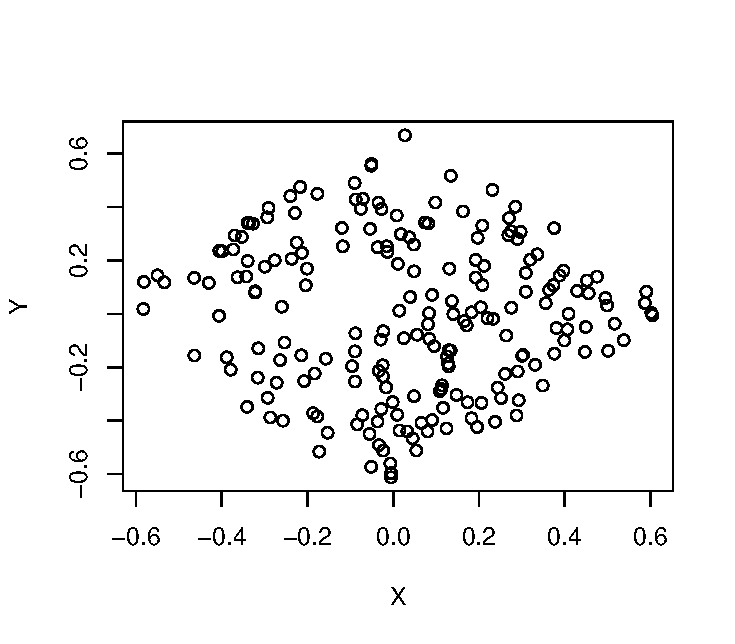
\includegraphics[width=\textwidth]{pics/XYplot}
\end{column}
\end{columns}
\begin{block}{Implication}
If economic data are heavy-tailed or nonlinear,
Pearson correlation can miss important structure.
\end{block}
\end{frame}


\begin{frame}[fragile]{Non-Gaussianity issue}
\begin{beamercolorbox}[wd=\paperwidth,sep=5pt]{important}
Vanishing covariance does not imply independence!
\end{beamercolorbox}
\begin{lstlisting}
# generate sample from two uncorrelated but dependent random variables
> set.seed(1); n <- 200
> A <- runif(n)-1/2; B <- runif(n)-1/2
> X <- t(c(cos(pi/4),-sin(pi/4)) %*% rbind(A,B))
> Y <- t(c(sin(pi/4),cos(pi/4)) %*% rbind(A,B))
> cor.test(X,Y, method = "pearson")

	Pearson's product-moment correlation

data:  X and Y
t = -0.84711, df = 198, p-value = 0.398
alternative hypothesis: true correlation is not equal to 0
95 percent confidence interval:
 -0.1971897  0.0793095
sample estimates:
        cor 
-0.06009275 \end{lstlisting}
$X$ and $Y$ are uncorrelated but dependent!
\end{frame}


%\begin{frame}[fragile]{Kendall's tau}
%Kendall's tau is a rank-based measure of association.
%
%\begin{block}{Definition}
%For a sample $(x_i,y_i)$, $(x_j,y_j)$:
%\begin{itemize}
%    \item they are \alert{concordant} if the order agrees in both coordinates,
%    \item they are \alert{discordant} if the order is reversed.
%\end{itemize}
%Then
%\[
%\tau=\frac{\#\text{concordant}-\#\text{discordant}}{\binom{n}{2}}.
%\]
%\end{block}
%
%\begin{lstlisting}
%set.seed(1)
%n <- 200
%Z <- runif(n)
%X <- runif(n)^2 + 0.4*Z
%Y <- runif(n)   + 0.4*Z
%
%cor.test(X, Y, method = "kendall")
%\end{lstlisting}
%
%\begin{alertblock}{Why use it?}
%It is more robust and still detects monotone dependence beyond the Gaussian setting.
%\end{alertblock}
%\end{frame}

\begin{frame}[fragile]{Distance correlation}
Distance correlation is a fully nonparametric measure of dependence.

\begin{block}{}
\textbf{Key property:}\qquad $
\mathcal R(X,Y)=0
\qquad\Longleftrightarrow\qquad
X\indep Y.
$\\[2mm]
\end{block}

\begin{lstlisting}
library(energy)
set.seed(1)
n <- 200
A <- runif(n) - 1/2
B <- runif(n) - 1/2
X <- A + B
Y <- A^2 - B^2

dcor.test(X, Y, R = 1000)
\end{lstlisting}

\begin{alertblock}{Interpretation}
This gives a permutation test for general dependence, not just linear or monotone association.
\end{alertblock}
\end{frame}

%\begin{frame}{Which test for which problem?}
%\begin{center}
%\begin{tabular}{l|l|l}
%\textbf{Method} & \textbf{Good for} & \textbf{Limitation} \\ \hline
%Pearson & linear / Gaussian dependence & misses nonlinear patterns \\
%Kendall & monotone dependence, robustness & not fully general \\
%Distance correlation & arbitrary dependence & heavier computationally
%\end{tabular}
%\end{center}
%
%\vspace{3mm}
%
%\begin{block}{Practical empirical message}
%The choice of test should reflect the kind of dependence you care about
%and the distributional features of the data.
%\end{block}
%
%\begin{alertblock}{Economic data reminder}
%Heavy tails, outliers, heteroskedasticity, and nonlinearities are common.
%So it is often worth going beyond Pearson correlation.
%\end{alertblock}
%\end{frame}

\begin{frame}[fragile]{Another cautionary example}
	Bowman\& Azzalini (1997) analyse aircraft wing span and speed data.	 
\begin{minipage}{5.2cm}
	\begin{lstlisting}
> library(sm); set.seed(1); 
> X <- aircraft$Span
> Y <- aircraft$Speed
> cor.test(X,Y)$p.value
[1] 0.7816014
> dcor.test(X,Y,R=1000)$p.value
[1] 0.000999001
\end{lstlisting}
\end{minipage}	\qquad\qquad\qquad 
	\begin{minipage}{7.2cm}
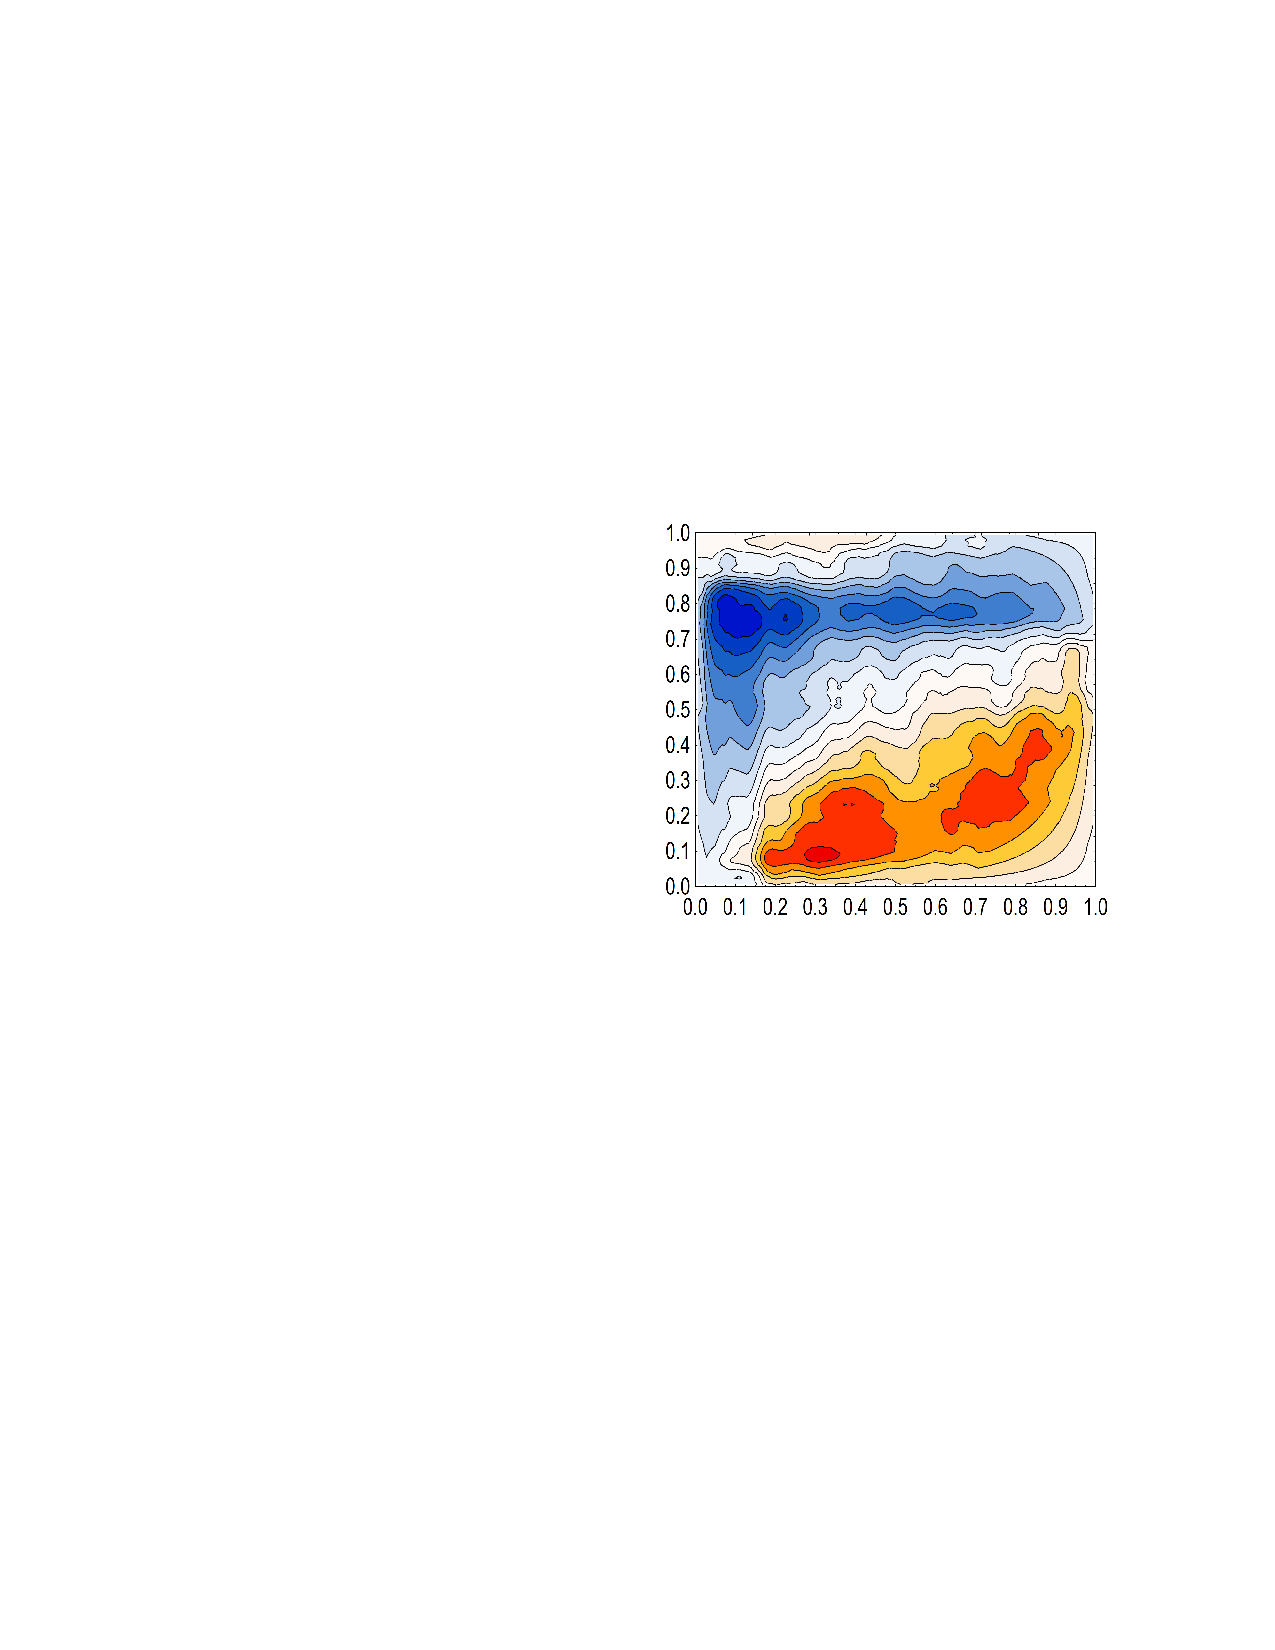
\includegraphics[scale=.6]{pics/aircraft}
\end{minipage}	

	
	 {\small For a discussion see: \'{C}miel, Ledwina, \textit{Validation of Association}, 2019. }
\end{frame}

\begin{frame}[fragile]{Tests for discrete data}
	\begin{alertblock}{$\chi^2$-test for discrete data}
   \begin{lstlisting}
> M <- as.table(rbind(c(762, 327, 468), c(484, 239, 477)))
> dimnames(M) <- list(gender = c("F", "M"),
+                     party = c("Democrat","Independent", "Republican"))

> (Xsq <- chisq.test(M))  # Prints test summary

	Pearsons Chi-squared test

data:  M
X-squared = 30.07, df = 2, p-value = 2.954e-07
     
> Xsq$expected   # expected counts under the null
      party
gender Democrat Independent Republican
     F 703.6714    319.6453   533.6834
     M 542.3286    246.3547   411.3166
      \end{lstlisting}
\end{alertblock}
\texttt{df = 2} is the difference between $5$ (saturated model) and $3$ (independence)
\end{frame}

\begin{frame}[fragile]{Testing conditional independence}
Testing
$
X \indep Y \mid Z
$
is \alert{much harder} than testing ordinary independence.
Once we condition on $Z$, we must compare \emph{conditional} laws rather than marginal ones.


\begin{columns}[T]
\begin{column}{0.58\textwidth}

\begin{block}{}
\small 
\begin{itemize}
    \item \textbf{Discrete data:} likelihood-ratio gives asymptotic $\chi^2$ procedures.\\[-2mm]
    \item \textbf{Gaussian data:} conditional independence reduces to zero partial correlation.\\[-2mm]
    \item \textbf{Nonlinear / non-Gaussian data:} kernel and other nonparametric methods are available, but they are computationally heavier.
\end{itemize}
\end{block}

\begin{beamercolorbox}[wd=\textwidth,sep=6pt,rounded=true,shadow=true]{important}\small 
In practice, the difficulty of CI testing depends strongly on the modelling assumptions.
\end{beamercolorbox}

\end{column}
\begin{column}{0.38\textwidth}

\begin{lstlisting}
library(CondIndTests)
library(bnlearn)
set.seed(1)

n <- 100
Z <- rnorm(n)
X <- 4 + 2*Z + rnorm(n)
Y <- 3*X^2 + Z + rnorm(n)

CondIndTest(X, Y, Z,
            method = "KCI")$pvalue
bnlearn::ci.test(X, Y, Z)$p.value
\end{lstlisting}
\vspace{-1mm}
\begin{alertblock}{Interpretation}
\scriptsize Here $X$ and $Y$ are \textbf{not} conditionally independent given $Z$,
so both procedures return very small $p$-values.
\end{alertblock}

\end{column}
\end{columns}

%\vspace{1mm}
%{\scriptsize For a broader discussion of nonlinear conditional independence testing, see Heinze-Deml, Peters, and Meinshausen (2018).}
\end{frame}

\begin{frame}[fragile]{Testing conditional independence in discrete data}

\begin{columns}[T,onlytextwidth]
\begin{column}{0.48\textwidth}
\textbf{Using \texttt{bnlearn}}
\begin{lstlisting}
library(gRim)
data(UCBAdmissions)

bnlearn::ci.test(
  x = "Gender",
  y = "Admit",
  z = "Dept",
  test = "x2",
  data = as.data.frame(UCBAdmissions)
)
\end{lstlisting}

\begin{lstlisting}
Pearson's X^2

data:  Gender ~ Admit | Dept
x2 = 0, df = 6, p-value = 1
alternative hypothesis:
true value is greater than 0
\end{lstlisting}
\end{column}

\begin{column}{0.48\textwidth}
\textbf{Using \texttt{gRim}}
\begin{lstlisting}
gRim::ciTest(
  as.data.frame(UCBAdmissions),
  set = ~ Gender + Admit + Dept
)
\end{lstlisting}

\begin{lstlisting}
Testing Gender _|_ Admit | Dept
Statistic (DEV): 0.000
df: 6
p-value: 1.0000
method: CHISQ

Slice information:
  statistic p.value df Dept
1         0       1  1    A
2         0       1  1    B
3         0       1  1    C
4         0       1  1    D
5         0       1  1    E
6         0       1  1    F
\end{lstlisting}
\end{column}
\end{columns}

\vspace{1mm}
\begin{beamercolorbox}[wd=\textwidth,sep=6pt,center,rounded=true,shadow=true]{important}
For this table, once we condition on department, there is no evidence that admission depends on gender.
\end{beamercolorbox}

\end{frame}

%\begin{frame}{A broader message for empirical work}
%Testing dependence is not just a statistical exercise.
%
%\begin{itemize}
%    \item In causal work, it tells us whether residual dependence remains after adjustment.
%    \item In finance and macro, it helps reveal dependence networks.
%    \item In high dimensions, it motivates sparse graphical models.
%\end{itemize}
%
%\vspace{2mm}
%
%\begin{beamercolorbox}[wd=\textwidth,sep=8pt,center,rounded=true,shadow=true]{important}
%Conditional independence is an abstract concept, but it leaves fingerprints in data.
%\end{beamercolorbox}
%\end{frame}

% ------------------------------------------------------------
% Closing
% ------------------------------------------------------------

\section{Conclusion}

\begin{frame}{Take-away}
\begin{itemize}
    \item Independence means factorization of the joint law.
    \item Conditional independence is a structural statement about what remains after conditioning.
    \item Conditioning can remove dependence, but it can also create it.
    \item In Gaussian models, conditional independence becomes algebraic:
    zeros in the precision matrix correspond to missing direct relations.
    \item Testing dependence requires care:
    Pearson and distance correlation target different notions.
\end{itemize}

\vspace{2mm}

\begin{beamercolorbox}[wd=\textwidth,sep=8pt,center,rounded=true,shadow=true]{important}
\textbf{Main lesson of today:}
to understand dependence, always ask what is being conditioned on.
\end{beamercolorbox}
\end{frame}

\begin{frame}{Looking ahead}
\begin{block}{Next lecture}
We will encode conditional independence statements visually using \imp{undirected graphs}.
\end{block}

\begin{alertblock}{What will come next?}
\begin{itemize}
    \item local, pairwise, and global Markov properties,
    \item Gaussian graphical models,
    \item sparse network estimation from data,
    \item applications to economic and financial dependence networks.
\end{itemize}
\end{alertblock}

\begin{center}
{\Large Missing edge $=$ conditional independence}
\end{center}
\end{frame}

\end{document}